\documentclass{standalone}
\usepackage{tikz}
\usepackage{pgfplots}
\pgfplotsset{compat=newest}
\usepackage{pgfmath}
\usepackage{tikz-cd}
\usepackage{pgffor}
\usepackage{tkz-euclide}
\usetkzobj{all}
\usepgfplotslibrary{fillbetween}
\usetikzlibrary{
	calc,
	angles,
	quotes,
	arrows.meta,
	decorations.markings,
	math,
	backgrounds,
	pgfplots.statistics,
	matrix,
	patterns,
	shapes.geometric,
	spy,
	intersections,
}
\begin{document}
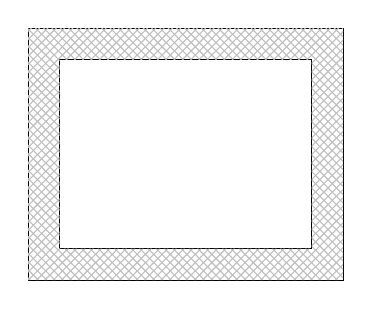
\begin{tikzpicture}[scale=0.8]
\draw[name path=outside]  (0,0)--(5,0)--(5,4)--(0,4)--cycle;
\draw[name path=inside] (0.5,0.5)--(4.5,0.5)--(4.5,3.5)--(0.5,3.5)--cycle;
\tikzfillbetween[
of=outside and inside,
] {pattern=crosshatch,pattern color=gray!50};
\end{tikzpicture}
\end{document}